%%%%%%%%%%%%%%%%%%%%%%%%%%%%%%%%%%%%%%%%%%%%%%%%%%%%%%%%%%%%%%%
%
% Welcome to Overleaf --- just edit your LaTeX on the left,
% and we'll compile it for you on the right. If you open the
% 'Share' menu, you can invite other users to edit at the same
% time. See www.overleaf.com/learn for more info. Enjoy!
%
%%%%%%%%%%%%%%%%%%%%%%%%%%%%%%%%%%%%%%%%%%%%%%%%%%%%%%%%%%%%%%%


% Inbuilt themes in beamer
\documentclass{beamer}

% Theme choice:
\usetheme{CambridgeUS}

% Title page details: 
\title{Assignment 7} 
\author{Varun Gupta \\ cs21btech11060}
\date{\today}
\logo{\large \LaTeX{}}


\begin{document}

% Title page frame
\begin{frame}
    \titlepage
\end{frame}

% Remove logo from the next slides
\logo{}


% Outline frame
\begin{frame}{Outline}
    \tableofcontents
\end{frame}
\section{Papoulis Solutions}
\begin{frame}{Problem}
    \begin{block}{Ex 2.27}
        We have two coins; the first is fair and the second two-headed. We pick one of the coins
        at random, we toss it twice and heads shows both times. Find the probability that the coin
        picked is fair.
    \end{block}
\end{frame}
\begin{frame}{Solution}
    \begin{block}{Solution:}
        Acoording to Bayes' theorem for two events A \& B:
        \begin{equation}
            P(A|B) = \frac{P(B|A) \cdot P(A)}{P(B)}
        \end{equation}
        Using Bayes' theorem:\\
            P(coin picked is fair) = $\frac{\frac{1}{4}}{\frac{1}{4}+2 \times \frac{1}{2}+1} = \frac{1}{9}$
    \end{block}
\end{frame}
\begin{frame}{Code}
    \begin{block}{Code:}
        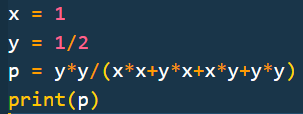
\includegraphics{figures/fig1.png}
    \end{block}
\end{frame}
\end{document}